\documentclass[12pt, a4paper]{memoir}

% Essential packages
\usepackage[T1]{fontenc}
%%\usepackage[latin1]{inputenc}
\usepackage[french,english]{babel}

% personal packages
\usepackage [includehead, margin=1.5cm]{geometry}                % See geometry.pdf to learn the layout options. There are lots.
\usepackage{graphicx} % include images
\usepackage{hyperref} % urls, hyperlinks, etc
% \usepackage{pdfpages} % include pdf pages
\usepackage{enumitem} % customize itemize
\usepackage[backend=bibtex]{biblatex} % bibliography
\usepackage{csquotes} % Quote bibliography and add hyperlinks
% \usepackage{titlesec} % Modify chapter headings
% \usepackage{wrapfig} % wrap text around figures
% \usepackage{float} % force figure positions at the end of the file
\usepackage[linesnumbered,ruled,vlined]{algorithm2e}

% Packages from uga template
%\usepackage{fullpage}
\usepackage{mathptmx} % font = times
\usepackage{helvet} % font sf = helvetica
% \usepackage{amsmath}
% \usepackage{relsize}
% \usepackage{tikz}
% \usepackage{booktabs}
% \usepackage{textcomp}%textquotesingle
% \usepackage{multirow}
% \usepackage{pgfplots}

% \usetikzlibrary{arrows,shapes,positioning,shadows,trees}
% \makesavenoteenv{tabular}
% \makesavenoteenv{table}

\def\checkmark{\tikz\fill[scale=0.4](0,.35) -- (.25,0) -- (1,.7) -- (.25,.15) -- cycle;}

%Style des têtes de section, headings, chapitre
\headstyles{komalike}
\nouppercaseheads
\chapterstyle{dash}
\makeevenhead{headings}{\sffamily\thepage}{}{\sffamily\leftmark} 
\makeoddhead{headings}{\sffamily\rightmark}{}{\sffamily\thepage}
\makeoddfoot{plain}{}{}{} % Pages chapitre. 
\makeheadrule{headings}{\textwidth}{\normalrulethickness}
%\renewcommand{\leftmark}{\thechapter ---}
\renewcommand{\chaptername}{\relax}
\renewcommand{\chaptitlefont}{ \sffamily\bfseries \LARGE}
\renewcommand{\chapnumfont}{ \sffamily\bfseries \LARGE}
\setsecnumdepth{subsection}
\addbibresource{biblio.bib}

% Customize itemize item markers
\renewcommand\labelitemi{-}

% Add source to figures caption
\newcommand*{\captionsource}[2]{%
    \caption[{#1}]{%
        #1%
        \\\hspace{\linewidth}%
	\textbf{Source:} \textit{#2}%
    }%
}

% Some settings for the title page
%\titleformat{\chapter}[display]{\normalfont\huge\bfseries}{}{0pt}{\Huge}
%\titlespacing*{\chapter} {0pt}{20pt}{40pt}

% Force footnotes to stay on one page
\interfootnotelinepenalty=10000

% Title page formatting -- do not change!
\newcommand{\HRule}{\rule{\linewidth}{0.5mm}}
\pretitle{\HUGE\sffamily \bfseries\begin{center}\HRule \\[0.2cm]} 
	\posttitle{\end{center}\HRule}
\preauthor{\LARGE  \sffamily \bfseries\begin{center}}
\postauthor{\par\end{center}}
\newcommand{\jury}[1]{% 
\gdef\juryB{#1}} 
\newcommand{\juryB}{} 
\newcommand{\session}[1]{% 
\gdef\sessionB{#1}} 
\newcommand{\sessionB}{} 
\newcommand{\option}[1]{% 
\gdef\optionB{#1}} 
\newcommand{\optionB} {}

\renewcommand{\maketitlehookd}{% 
\vfill{}  \large\par\noindent  
\begin{center}\juryB \bigskip\sessionB\end{center}
\vspace{-1.5cm}}
\renewcommand{\maketitlehooka}{% 
	\vspace{-1.5cm}\noindent
\includegraphics[height=12ex]{../imgs/uga-logo.png}\hfill\raisebox{2ex}{
\includegraphics[height=14ex]{../imgs/ENSIMAG.png}}\\
\bigskip
\begin{center} \large
Master of Science in Informatics at Grenoble \\
Master Informatique \\ 
Specialization \optionB  \end{center}\vfill}
% =======================End of title page formatting

\option{MoSIG} 
\title{Simulation of a Kubernetes Cluster with Validation in Real Conditions} %\\\vspace{-1ex}\rule{10ex}{0.5pt} \\sub-title} 
\author{LARUE Théo}
\date{Defense Date, 2020} % Delete this line to display the current date
\jury{
	Research project performed at Laboratoire d'Informatique de Grenoble \\\medskip
Under the supervision of:\\
Michael Mercier\\\medskip
Defended before a jury composed of:\\
Head of the jury\\
Jury member 1\\
Jury member 2\\
}
\session{September \hfill 2020}
\setcounter{tocdepth}{4}
\setcounter{secnumdepth}{4}

\begin{document}
\selectlanguage{english} % french si rapport en français
\frontmatter
\begin{titlingpage}
\maketitle
\end{titlingpage}

%\small
\setlength{\parskip}{-1pt plus 1pt}

\renewcommand{\abstracttextfont}{\normalfont}
\abstractintoc
\begin{abstract} 
	The rise of containerized applications has provided web platforms with
	much more control over their resources than they had before with their
	physical servers. Soon enough, developers realized they could go even
	further by automating container management operations to allow for even
	more scalability. The Cloud Native Computing Foundation was founded in
	this context, and developed Kubernetes which is a piece of software
	capable of container orchestration, or in other words, container
	management. Now, as we observe a convergence between HPC (High
	Performance Computing) and the Big Data field where Kubernetes is
	already the standard for some applications such as Machine Learning,
	discussions about leveraging containers for HPC applications rose and
	interest in Kubernetes has grown in the HPC community. One of the many
	challenges the HPC world has to face is scheduling, which is the act of
	allocating tasks submitted by users on available resources. In order to
	properly evaluate and develop schedulers researchers have used
	simulators for decades to avoid running experiments in real conditions,
	which is costly both in time and resources. However, such simulators do
	not exist for Kubernetes or are not open to the public. While the
	default scheduler works great for most of the Cloud Native
	infrastructures Kubernetes was designed for, some teams of researchers
	would rather be able to experiment with different batch processing
	policies on Kubernetes as they do with traditional HPC. Our goal in
	this master thesis is to describe how we developed Batkube, which it is
	an interface between Kubernetes schedulers and Batsim, a general
	purpose infrastructure simulator based on the Simgrid framework and
	developed at the LIG.

\end{abstract}
\abstractintoc

\renewcommand\abstractname{Acknowledgement}
\begin{abstract}
I would like to express my sincere gratitude to .. for his invaluable assistance and comments in reviewing this report... 
Good luck :) 
\end{abstract}

\renewcommand\abstractname{R\'esum\'e}
\begin{abstract} \selectlanguage{french}
	Abstract mais en franchais
\end{abstract}
\selectlanguage{english}

\tableofcontents* % the asterisk means that the table of contents itself isn't put into the ToC
\normalsize

\mainmatter
\SingleSpace

\chapter{Introduction}
\section{Scheduling and simulators}
\subsection{A bit of context : High Performance Computing}

TODO

A general definition of HPC would be :
``\textit{High Performance Computing (HPC) most generally refers to the
		practice of aggregating computing power in a way that delivers
		much higher performance than one could get out of a typical
		desktop computer in order to solve large problems in science,
		engineering, or
		business.}
\footnote{\url{https://wwwen.uni.lu/university/high_performance_computing}}''.
HPC can either refer to ``High Performance Computing'' or ``High Performance
Computer'' but it is generally clear which one it refers to, given the
context.

A HPC workload is composed of numerous tasks hungry for computational resources
which are executed in parallel on different machines (that we can refer to as
compute resources or nodes). These tasks may be completely independant like
when different users each submit a single task, or they may also be tightly
coupled together as when a single user submits a job that is composed of
several tasks than can be run in parallel. In that case, the whole system
becomes very sensitive to latency as these tasks have got to communicate
together. This is done through MPIs (Message Passing Interfaces) which
represent a large part of the HPC field.\\

\subsection{The scheduling problem}
\begin{displayquote}[][]
	\textbf{schedule} \textit{n.} : A plan for
	performing work or achieving an objective, specifying the order and
	allotted time for each part.
\end{displayquote}

In a general way, scheduling is the concept of allocating available resources
to a set of tasks, organizing them in time and space (the resource space). The
resources can be of any nature, and the tasks independant from each others or
linked together.

In computing the definition remains the same, but with automation in mind.
Schedulers are algorithms that take as an input either a pre-defined workload,
which is a set of jobs  to be executed - the tasks are called jobs in this
context -, or simple jobs submitted over time by users in an unpredictable
manner. In the latter case, the jobs are added to a queue managed by the
scheduler. Scheduling is also called batch scheduling or batch processing, as
schedulers allocate batches of jobs at a time. Jobs are allocated on machines,
virtual or physical, with the intent of minimizing the total execution time,
equally distributing resources, minimizing wait time for the user or reducing
energy costs. As these objectives often contradict themselves, schedulers have
to implement compromises or focus on what the user really needs or requires.  

The scheduler has many factors to keep in mind while trying to be as efficient
as possible, such as :

\begin{itemize}
	\item Resource availability and jobs resource requirements
	\item Link between jobs (some are executed in parallel and need synchronization, some are independant)
	\item Latency between compute resources
	\item Compute resources failures
	\item Jobs priority
	\item Machine shutdowns and restarts
	\item Data locality
\end{itemize}

All these elements make scheduling a very intricate problem that is at best
polynomial in complexity, and often NP-hard\cite{scheduler-complexity}.
Moreover, with the growing complexity of modern RJMS\footnote{The RJMS
	(Resource and Job Management System) is the software at the core of the
	cluster. It is a synonym for a scheduler and manages resources, energy
	consumption, users' jobs life-cycle and implements scheduling
	policies.} and the wide variety in infrastructures, scheduler
performances are rather inpredictable.

\subsection{The need for an infrastructure simulator}
 
TODO 

The complexity of the schedulinng problem and the high cost of running real
world scenarios makes the use of a simulator almost mandatory when evaluating
scheduling policies or developing a new scheduler. Indeed, modeling a scheduler
and its interactions with a given infrastructure and workload is far too
difficult for modern software and infrastructure.

\section{Batsim}

\section{Kubernetes}
\subsection{Kubernetes overview}
\subsubsection{Cloud Native Computing}
In the early stages of application development, organizations used to run their
services on physical servers. With this direct approach came many challenges
that needed to be coped with manually like resources allocation,
maintainability or scalability. In an attempt to automate this process
developers started using virtual machines which enabled them to run their
services regardless of physical infrasctucture while having a better control
over resources allocation.  This led to the concept of containers which takes
the idea of encapsulated applications further.

\begin{figure}[h]
	\centering
	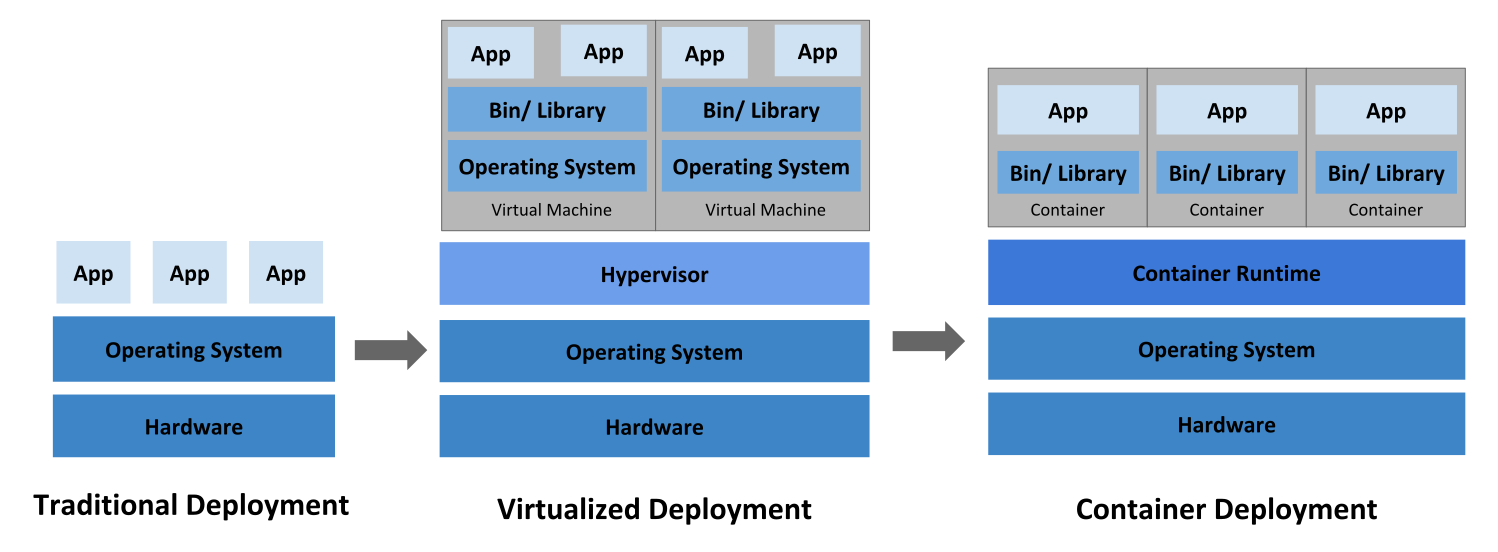
\includegraphics[width=\textwidth]{../imgs/container_evolution.png}
	\captionsource{Evolution of application deployment.}{https://kubernetes.io/docs/concepts/overview/what-is-kubernetes/}
	\label{fig:container-evolution}
\end{figure}

Containers can be thought of as lightweight virtual machines. Unlike the
latter, containers share the same kernel with the host machine but still allow
for a very controlled environment to run applications. There are many
benefits to this : separating the development from deployment, portability,
easy resource allocation, breaking large services into smaller micro-services
or support of continuous integration tools (containers greatly facilitate
integration tests).\\

The CNCF\footnote{\url{https://www.cncf.io/}} (Cloud Native Computing
Foundation) was founded in the intent of leveraging the container technology
for an overall better web. In a general way, we now speak of these
containerized and modular applications as cloud native computing :

\textit{``Cloud native technologies empower organizations to build and run
	scalable applications in modern, dynamic environments such as public,
	private, and hybrid clouds. Containers, service meshes, microservices,
	immutable infrastructure, and declarative APIs exemplify this
	approach.}

\textit{These techniques enable loosely coupled systems that
	are resilient, manageable, and observable.  Combined with robust
	automation, they allow engineers to make high-impact changes frequently
	and predictably with minimal toil.``}\footnote{\url{https://github.com/cncf/toc/blob/master/DEFINITION.md}}

Kubernetes\footnote{\url{https://kubernetes.io/}} is the implementation of this
general idea and was anounced at the same time as the CNCF. It aims at
automating of the process of deploying, maintaining and scaling containerized
applications. It is industry grade and is now the de-facto solution for
container orchestration.


\subsubsection{Kubernetes concepts}
The basic processing unit of Kubernetes is called a \textbf{pod} which is
composed of one or several containers and volumes\footnote{A volume is some
	storage space on the host machine that can be linked to containers, so
	they can read persistent information or store data in the long term}.
In the cloud native context a pod most often hosts a service or micro-service.

\begin{figure}[h]
	\centering
	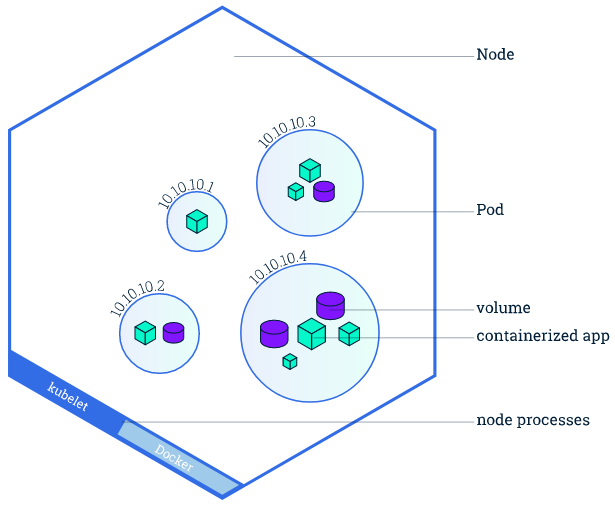
\includegraphics[scale=0.5]{../imgs/node-overview.png}
	\captionsource{Node overview}{https://kubernetes.io/docs/tutorials/kubernetes-basics/explore/explore-intro/}
	\label{fig:node-overview}
\end{figure}

Pods are bundled together in \textbf{nodes} (figure \ref{fig:node-overview})
which are either physical or virtual machines. They represent another barrier
to pass through to access the outside world which can be useful to add layers
of security or facilitate communication between pods. Nodes take the idea of
containerisation further by encapsulating the already encapsulated services.
Each node runs at least one pod and also one \textbf{kubelet} which is a
process responsible for communicating with the rest of Kubernetes (or more
precisely, with the master node which in turns communicates with the api
server). A set of nodes is called a \textbf{cluster}. Each Kubernetes instance
is responsible for running a cluster.

Kubernetes revolves its API server which is its central component (figure
\ref{fig:kube-components}). The majority of operations between components go
through this REST API like user interactions through kubectl or scheduling
operations.

\begin{figure}[h]
	\centering
	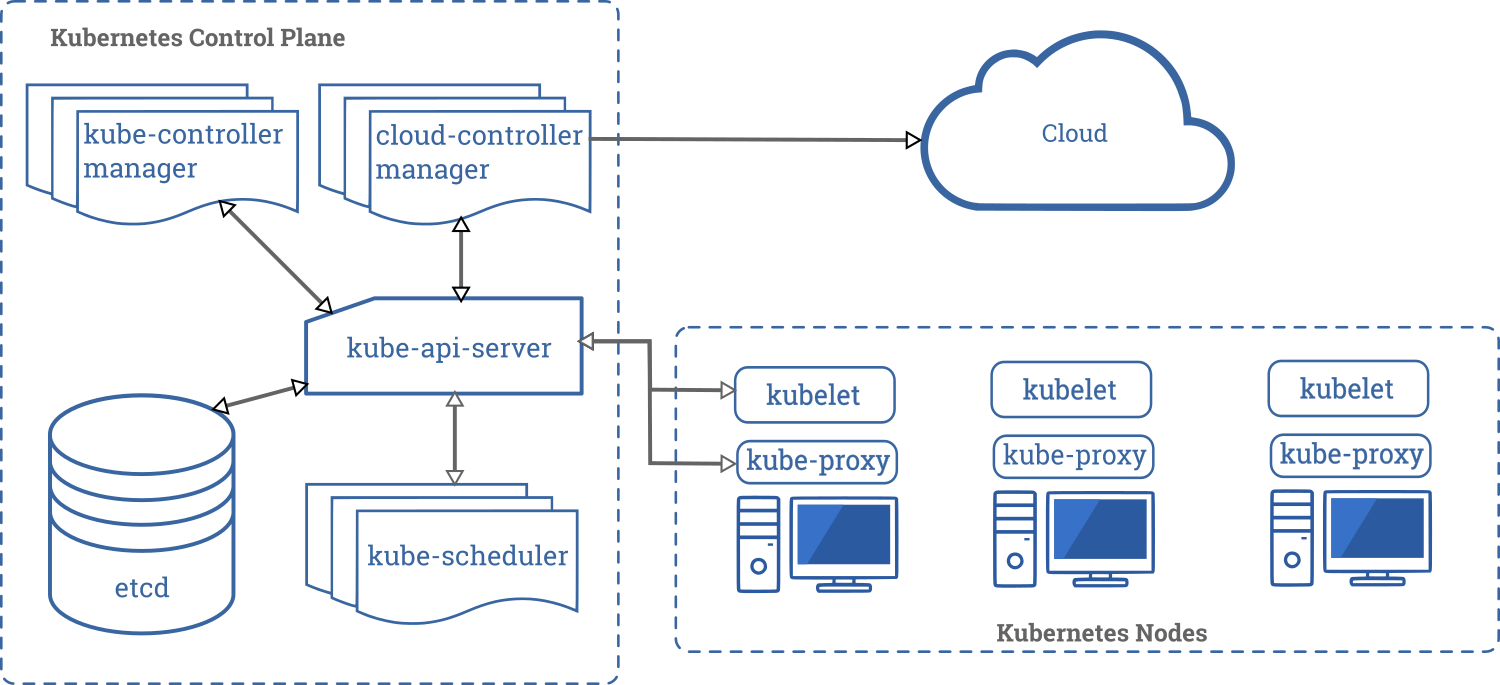
\includegraphics[width=\textwidth]{../imgs/components-of-kubernetes.png}
	\captionsource{Components of Kubernetes}{https://kubernetes.io/docs/concepts/overview/components/}
	\label{fig:kube-components}
\end{figure}

\newpage % hotfix for problematic figure placement
\subsection{HPC and Kubernetes}
The difference between HPC and Cloud Native computing lies in the workloads
they are intended to tackle.  Kubernetes was designed for Cloud Native
applications. Services or micro services are run in containers and are expected
to be available at all times : they are replicated as many times as the user
desires and restarted whenever a failure occurs. High availability is at the
core of Kubernetes container management.  On the other hand, depending on
scheduling policies, HPC is focused on user wait time, maximizing resource
usage, optimizing energy costs... For instance, in case of failure, it is
sometimes not sufficient to restart the single job that failed : the entire
submission must be re-run if it is part of several jobs computed in parallel.

Kubernetes is now the standard for AI and Machine Learning as shown by the many
efforts at making this coupling an efficient
environment\cite{lee2017design}\cite{233001}\cite{10.1145/3154842.3154845},
which brought an increasing interest for container driven HPC aswell and
Kubernetes for HPC in particular. Batch schedulers such as
kube-batch\footnote{\url{https://github.com/kubernetes-sigs/kube-batch}} have
been implemented for kube, and numerous HPC applications like
slurm\footnote{\url{https://slurm.schedmd.com/containers.html}} now support containers as well.

Indeed, containers have many advantages that HPC users can benefit from. Here
are some notable ones:
\begin{itemize}
	\item First off, research has shown that Kuberenetes offer similar
		performance to more standard bare metal HPC\cite{8950981}.
	\item Users will get the same environment everywhere making up for a
		uniform and standardized workplace.
	\item Portability : users could seamlessly hop from one infrastructure
		to another based on their needs and criteria like price,
		performance, and capabilities rather than compatibility.
	\item Encapsulation : HPC applications often rely on complex
		dependencies that can be easily concealed into containers.
\end{itemize}
\begin{figure}[h]
	\centering
	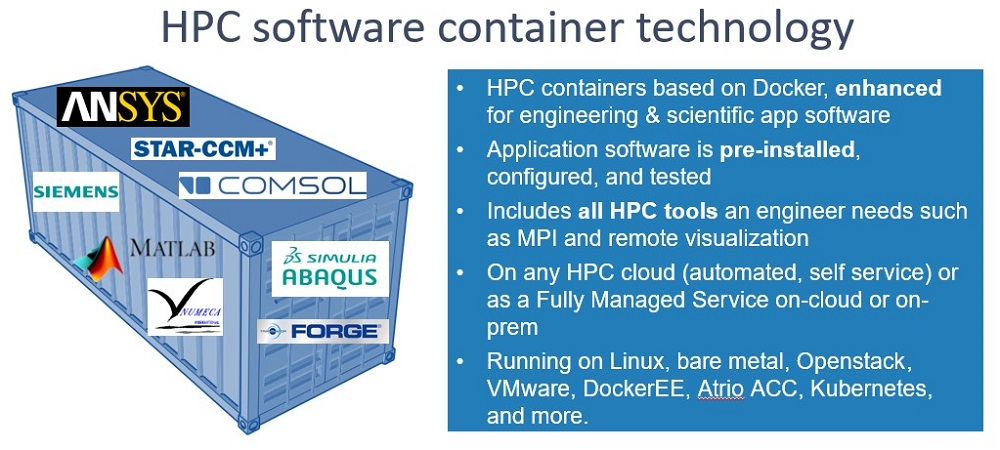
\includegraphics[scale=0.5]{../imgs/hpc-container.jpg}
	\captionsource{The container technology for HPC}{https://www.hpcwire.com/2019/09/19/kubernetes-containers-and-hpc/}
	\label{fig:hpc-container}
\end{figure}

Despite all those advantages, Kubernetes is not ready yet to be used in proper
HPC environment because it lacks vital components like a proper batch job
queuing system, and support for MPI applications. It cannot yet compete against
the very well established HPC ecosystem, but that time may come soon as
containers are becoming more and more integrated in modern infrastructures.

\chapter{State of the art}
\section{Infrastructure simulators}

Developing a scheduler implies being able to test its performances throughout
the development process, however, testing in real conditions is time consuming
and expensive.  Organizations can either have enough resources to cover these
costs, or test their scheduler against a simulation.\\

Kubernetes cluster simulations is an open problem and is the subject of this
master project. Our approach relies on the Batsim\cite{batsim} infrastructure
simulator, which is itself built upon Simgrid\cite{simgrid}. Batsim is
currently mostly used to simulate HPC infrastructures but was designed to be
able to simulate any kind of infrastructure and therefore is theoretically able
to simulate any Kubernetes cluster, moreover, Kubernetes was designed to run
services but is capable of handling High-Performance
Computing\cite{kube-for-hpc}. This project aims at adapting Batsim so it can
evaluate Kuberenetes schedulers.

\section{Kubernetes schedulers}

\subsubsection{kube-scheduler}
Not exactly a batch scheduler, it is the default scheduler for Kubernetes made
by the CNCF"" --> "hop là"
\subsubsection{kube-batch}
\subsubsection{Poseidon}
\subsubsection{bashScheduler by rothgar}
\subsubsection{random-scheduler by Banzaicloud}
\subsubsection{k8s-custom-scheduler by IBM}
\subsubsection{scheduler by kelseyhightower}

\chapter{Problematic}

\section{Objectives}

The goal of this project is to design and implement Batkube, which will be an
interface between Batsim and Kubernetes schedulers. With this interface, we
want to compare Batsim results gainst data from a real Kubernetes cluster,
given HPC workloads.

\section{Translation}

\section{Synchronization}

\chapter{Implementation}

\section{Batkube architecture}
TODO

\section{API implementation}
\section{Time hijack}
TODO

\subsection{batsky-go}
\SetKwInput{KwInput}{Input}
\SetKwInput{KwOutput}{Output}


\begin{algorithm}[H]
\DontPrintSemicolon
\KwInput{req: request channel, res: result channel map}
\While{Batkube is not ready} {
	wait\;
}
requests = []request\;
\While{req is not empty} {
	m = $<$- req \tcc{Non blocking receive}
	requests = append(requests, m)\;
}
sendToBatkube(requests) \tcc{Only requests with duration > 0 are actually sent. Batkube will always anwser.}
now = responseFromBatkube()\;
\For{m in range requests} {
	res[m.id] $<$-now \tcc{The caller continues execution upon reception}
}

	
\caption{Requester loop}
\label{alg:reqLoop}
\end{algorithm}


\begin{algorithm}[H]
\DontPrintSemicolon
\KwResult{Current simulation time}
\KwInput{d: timer duration, req: request channel, res: response channel map}
\KwOutput{now : simulation time}

\If{requester loop is not running}{
	go runRequesterLoop() \tcc{There can on ly be one loop runing at a time}
}
id = newUUID()\;
m = newRequestMessage(d, id) \tcc{Requests are identified using uuids}
resChannel = newChannel()\;
res[id] = resChannel \tcc{A channel is associated with each request}
req $<$- m \tcc{The code blocks here until request is handled}
now = $<$-resChannel \tcc{The code blocks here until response is sent by the requester loop}
return now\;
\caption{Time request (time.now())}
\label{alg:now}
\end{algorithm}



\chapter{Evaluation}

\chapter{Conclusion}


\backmatter
\printbibliography
\end{document}
